\chapter{Dynamics of nucleosomal DNA}
\label{sec:nucleosome}
Every cell of a multicellular organism carries the complete genetic information in its genome, 
regardless of its specific role as a part of the whole. Since different cells, \emph{e.g.}~a liver cell
and a neuron, need different proteins to function, cells are in need of a mechanism to control
which part of the genome is transcribed and which genes are silent. This not only applies to 
specialized cells of multicellular organisms, but to every cell we know. Even the simplest bacteria 
need to adjust their metabolism to the available nutrients and require different proteins at
different stages of the cell cycle. Regulation of protein production can occur either before
the gene is transcribed into mRNA, or target the process of the translation of mRNA 
into protein. 
To regulate transcription, the DNA contains short sequences that bind specifically to 
proteins called \emph{transcription factors} (TF). These transcription factors repress or
enhance the binding of the polymerase to the promoter, which is 
a prerequisite for transcription. The expression levels of the cell's genes is thereby 
controlled by the concentrations of transcription factors in the cell.

Eukaryotic cells suffer from an additional difficulty in achieving this feat. To fit their DNA into the 
cell's nucleus, the DNA needs to be strongly compactified. Due to this compactification the DNA is 
no longer freely accessible and transcription factor binding to DNA is to some extent precluded. 
The precise mechanisms of transcription regulation
in eukaryotes are unknown, but there is evidence that the compactified DNA is dynamic enough and 
exposes each part of its genome sufficiently often to allow for TF binding. 
On the other hand, cells exploit DNA compactification to
silence subsets of their genes and to determine cell fates during development. 
The dynamics of the elementary compactification unit of eukaryotic DNA, the nucleosome, has recently
been tested experimentally. In order to understand how the observed dynamics depends 
on various parameters of the system and what physical mechanisms might be responsible 
for the observed behavior, we investigate the dynamics of nucleosomes theoretically using
a simple model. Within our model, the dynamics of nucleosomes depends drastically on the 
polymer properties of DNA, which could also hold true for their dynamics \emph{in vivo}. 

In this chapter, I want to discuss the basics of chromatin structure and its implications
for gene regulation in eukaryotes. Then we will discuss two recent experiments, that studied the 
dynamics of nucleosomes and close with a discussion of our theoretical study.
%, that addresses the kinetics 
%of thermally activated DNA unwrapping from nucleosomes. 


%% CHECK NUMBERS IN FOLLOWING PARAGRAPH
\section{DNA compactification}
While bacteria have small genomes and avoid superfluous DNA, eukaryotes and in particular higher
multicellular organisms need more room to store their genetic information. In addition to the  
greater number of proteins that need to be coded, eukaryotes also tend to 
accumulate DNA that does not code for proteins and whose function is still unclear. In any case, 
the genomes of eukaryotes can be as big as a few gigabases for higher mammals. Even if broken 
up into several chromosomes, a DNA coil of that length is several tens of micrometers in diameter,
which is larger than the cell nucleus. Hence, there is a need for compactification, which is achieved
by an elaborate hierarchical organization of the DNA into chromosomes, as sketched in
\FIG{chromosome_organization}. 

At the lowest level of organization, the DNA double helix is wrapped
around a protein complex of cylindrical shape with a diameter of about 6~nm. This elementary packing unit is commonly 
referred to as a nucleosome. Its structure is known in exquisite detail and will be discussed in \SEC{nuc_structure}.
\begin{figure}
\centering
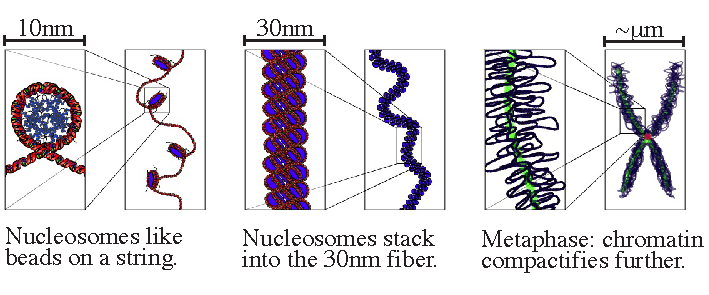
\includegraphics[width=\largefigure]{\FIGPATH/Figures_nucleosome/chromatin_structure}
\caption[Hierarchical organization of chromatin.]{\label{fig:chromosome_organization}
DNA is compactified into chromosomes in a hierarchic manner. See main text for details. 
%At the lowest level, DNA
%is wrapped around cylindrical proteins complex. The DNA-protein complexes are called
%nucleosomes. DNA with regularly spaced nucleosomes stacks into a thick and flexible fiber
%with 30nm in diameter. The structure at length scales between 100nm and $\mu m$ is less well known.
%Only during metaphase, dense chromosomes are formed. 
Image source: Wikipedia.}
\end{figure}
Nucleosomes are more or less evenly spaced on the genome with an average distance of about 30~nm. 
When stretched or in low salt conditions, this structure looks like a string of DNA with beads, 
the nuclesosomes, of about 10~nm in diameter. 
Under physiological conditions, this array of nucleosomes is further compactified to form a fiber  with 
30~nm in diameter, the structure of which is still subject to debate. The two competing models 
differ primarily in the geometry of the linker DNA between consecutive nucleosomes. In \emph{solenoid}
models, it is assumed that nucleosomes are arranged along a helix \cite{Finch_PNAS_76}, which 
requires the linker DNA between two nucleosomes to be strongly bent. For the second class of models,
it is assumed that the linker DNA is straight and crosses the center of the chromatin fiber. In 
these \emph{zig-zag} models two consecutive nucleosomes are assumed to lie on more or 
less opposite sides of the fiber \cite{Woodcock_PNAS_93}. Recently, the crystal structure
of tetra-nucleosomes was resolved, providing evidence for a zig-zag structure \cite{Dorigo_Science_04, Schalch_Nature_05}. A computational study also suggests
that the structure of oligo-nucleosomes is best described by an irregular zig-zag model \cite{Arya_PNAS_06}.
A more comprehensive overview and a survey of the current state of the debate is given in \REF{Woodcock_CurrOpStructBio_06}.
Due to its stacked structure without strong interactions along the direction of the fiber, the chromatin 
fiber is rather flexible and easily ripped apart by longitudinal tension. Stretching experiments on a single
chromatin fiber and comparison to an extensible worm-like-chain model suggest a persistence length 
of about 30~nm and a stretching modulus of 5pN \cite{Cui_PNAS_00}. This experiment further indicates, that 
the chromatin fiber disintegrates if tensions beyond 20pN are applied. 
Little is known about the intermediate levels of chromatin organization. It is believed, that the 30~nm fiber
forms large loops that are arranged on some scaffold, but evidence is sparse \cite{Alberts_02}. 
Only during cell division in the so called metaphase,  the DNA is packed into the dense structure known 
as chromosome\footnote{The name chromosome is derived from the greek word \emph{chromos} for 
color, since chromosomes are easily stained with dyes that bind to DNA.} that is large enough to be seen in
the light microscope. Our focus here is on the elementary packing unit, the nucleosome, and we will 
therefore describe the structure of the nucleosome in greater detail.

\subsection{\label{sec:nuc_structure}The nucleosome core particle}
While the structure of chromatin at larger length scales is still under debate, the nucleosome
 has been studied at atomic resolution. \citeauthor{Luger_Nature_97} succeeded 
in crystalizing the complex of histone proteins together with a short piece of DNA  wrapped around 
the protein complex 	and resolved the structure using X-ray scattering techniques. The first study achieved
a resolution of 2.8$\Ang$ \cite{Luger_Nature_97} and a subsequent experiment improved the resolution
to 1.9$\Ang$ \cite{Davey_JMB_02}. The structure of the nucleosome is illustrated in \FIG{nuc_structure}.
A piece of DNA, precisely 147~bps long, is wrapped around a cylindrical protein complex 1.7 times along 
a left-handed super-helical path. The pitch of this path is only 2.8~nm, such that the DNA comes very close
to itself along the super-helix. The protein complex has a diameter
of 6.5~nm and a height of about 6~nm. The cylinder is assembled out of four different  histone proteins
H2A, H2B, H3 and H4, each of which is present in two copies. 
These proteins form crescent shaped heterodimers (H2A-H2B) and (H3-H4), 
which are arranged such that they define a binding path for the DNA. 
\begin{figure}
\centering
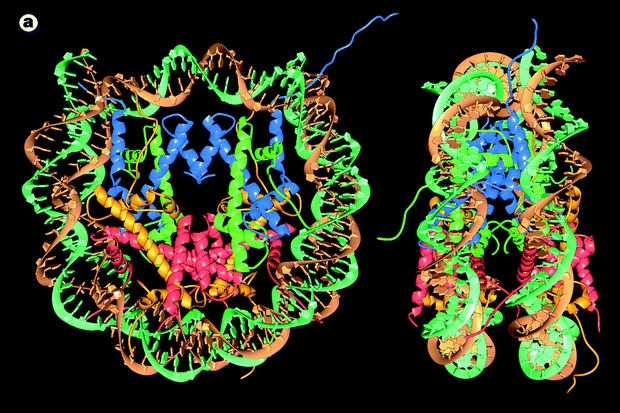
\includegraphics[width=\largefigure]{\FIGPATH/Figures_nucleosome/nucleosome_crystalstructure}
\caption[Crystal structure of Nucleosomes]{\label{fig:nuc_structure} The nucleosome consists of 147~bp of DNA wrapped 1.7 times around
a complex of eight proteins. The two strands of DNA are shown in turquoise and brown. Only the 
main chains of the histone proteins are shown (H3: blue, H4: green, H2A: yellow, H2B: red).
Figure reprinted with kind permission by Nature \cite{Luger_Nature_97}.}
\end{figure}
The histone complex is positively charged and therefore attracts the negatively charged DNA. 
The DNA-protein interaction is concentrated in 14 well defined contact points located at positions where the minor 
groove of the DNA faces the protein core. Each contact points forms a variable number of hydrogen bonds with the
DNA. Due to the electrostatic nature of the protein-DNA interaction, 
the stability of nucleosomes depends on salt concentration.
With increasing salt concentration, nucleosomes disassemble into DNA and the histone core complex, before
the histone complex dissociates further into the dimers \cite{Schiessel_JPhysCondMat_03}.

The net binding free energy between DNA and the 
histones can be estimated using cleavage enzymes that cut DNA at specific sites. In these experiments,
cleavage sites are placed at different locations on the wrapped DNA and the reduction of 
the cleavage rate compared to free DNA is measured. By measuring this rate reduction,
one can estimate the fraction of time the DNA site is accessible to protein binding 
\cite{Polach_JMB_95, Polach_JMB_96, Anderson_JMB_00}, from which the free energy difference
of the wrapped and the unwrapped state is calculated. 
These cleavage studies also revealed a significant sequence dependence 
of the net binding energies, but as a rule of thumb, each contact point contributes about
1.5 to 2$\kT$ to the net binding free energy under physiological conditions. The net binding free energy is the amount 
by which the total interaction energy exceeds the free energy needed to force the DNA into
the strongly bent and clamped conformation when wrapped around a histone complex. 
The latter can be estimated as follows.
When only moderately bent, dsDNA is well described by a worm-like-chain model (WLC, comp. \SEC{stretching_dsDNA})  for semi-flexible
polymers with a persistence length of $\lp=50\nm$. Within the WLC model, the bending energy 
of the DNA in a nucleosome can be estimated to 
\begin{equation}
\label{eq:DNA_bending_energy}
E_{bend}=\kT\frac{\lp l}{2R^{2}}\approx 58\kT,
\end{equation}
where $R=4.3\nm$ is the radius of curvature of the DNA contour and  $l=43\nm$ is the length of the bend part.
%which is slightly shorter than the total length, since the last 3~nm on both strands are essentially straight.
This number for $E_{bend}$ should only be considered as an order of magnitude estimate, since 
it is not at all clear whether the WLC model is applicable to strongly bent DNA.
The estimate for the bending free energy leads to an estimate of the total interaction free energy of 
about $6\kT$ per contact point.  The binding strength and the bendability of the DNA are strongly
sequence dependent and special sequences, called positioning sequences, 
are known to bind preferentially to histones in a precise alignment.

\section{Gene regulation in eukaryotes}
In prokaryotes, the set of genes which is transcribed by the RNA polymerase into mRNA 
is determined by the concentration of transcription factors (TF) in the cytosol. 
The regulatory sequences to which TFs bind specifically are usually located
from 20 to a couple of hundred base pairs upstream of the gene and either enhance the 
binding of the polymerase to the promoter site by attractive interaction
or prevent the binding of the polymerase by steric hinderance. 
%Signals associated with different
%TFs can be logically combined by TF interaction and suitable architecture
%of the regulatory sequence \cite{Gerland_PNAS_02, Buchler_PNAS_03}.
These regulatory mechanisms are well established for prokaryotes, where the DNA is freely accessible
to passive TFs. 

Transcription regulation in eukaryotes is more complicated and many additional stages of regulation exist. 
The regulatory sites for a specific gene can be far away from the site where transcription starts and many more
signals are integrated to determine whether a gene is to be silent or not. The general picture of eukaryotic 
gene regulation is far from complete. Nevertheless, TFs have to find their binding sites,
even if they are hidden by nucleosomes. The comparatively small net binding 
energy of nucleosomes led to the hypothesis, that transient unwrapping of DNA from the histone complex
driven by thermal fluctuations could suffice for reliable gene regulation \cite{Polach_JMB_96}. 
\citeauthor{Polach_JMB_96} coined the term \emph{site exposure mechanism} for this tentative 
mode of gene regulation. The mechanism is illustrated in \FIG{site_exposure_mechanism}a. 
\begin{figure}
\centering
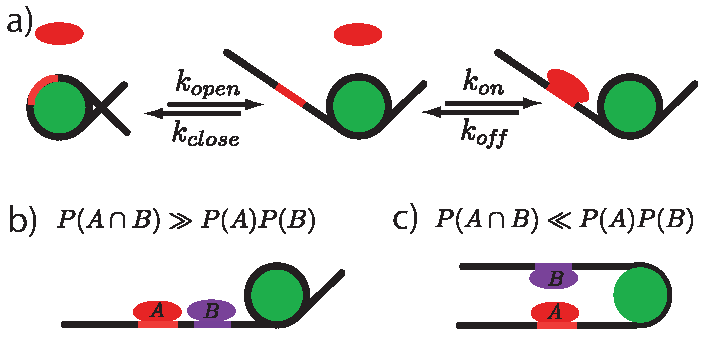
\includegraphics[width=\smallfigure]{\FIGPATH/Figures_Nucleosome/site_exposure_mechanism}
\caption[Site exposure mechanism]{\label{fig:site_exposure_mechanism}
Site exposure mechanism for protein binding to nucleosomal DNA.
Part a): Before the protein (red blob) can bind to its binding site (red), the DNA (black) has to detach from 
the histone complex (green). 
Part b\&c): Nucleosomes can mediate transcription factor interactions, see main text. 
%If two binding sites are located on the same side of the nucleosome dyad, their joint
%binding probability is greater than the product of the individual binding probabilities. 
%Part c): The converse is true, if the binding sites are located on opposite ends of the nucleosome,
%since unwrapping the last DNA turn is more costly than the first 0.7 turns due to the lack of electrostatic
%self repulsion of DNA.
}
\end{figure}
The site exposure mechanism allows to tune the binding affinity of a TF
 by the location of the binding site inside the nucleosome, the further away a site is from the 
entry or exit point, the harder it is to access. Indeed, it has been shown that the positioning
of nucleosomes along the genome is carefully controlled \cite{Segal_Nature_06}, which might be 
related to the tuning of binding affinities of TFs to their sites. The nucleosome can also be exploited
to mediate indirect interactions between TFs, see \FIG{site_exposure_mechanism}b\&c.
If two binding sites are located on the same side of the symmetry point of the nucleosome, exposure
of the binding site further inside the nucleosome implies the exposure of the other. Hence, the
joint binding probability is higher than the product of the individual binding probabilities, which is
equivalent to cooperative binding of the TFs. This type of nucleosome mediated TF interaction has
been shown to be a functional mode of gene regulation \emph{in vivo} \cite{Miller_MolCellBiol_03}.
In the opposite case, where the two sites
are at different ends of the piece of DNA, simultaneous binding is disfavored. To rationalize this, recall that
DNA is highly charged. In a nucleosome, DNA is wrapped 1.7 times along a helical path such that the  
DNA comes very close (a few \Ang) to itself for 0.7 turns. Due to self-repulsion of DNA, the first
0.7 turns are rather easy to unwrap, while the final turn is much more stable since self repulsion is
lacking. Two binding sites on opposite ends of the DNA are usually individually accessible by unwrapping
less than 0.7 turns of DNA, however, when exposing both of them simultaneously only little DNA remains
wrapped and one has to compensate the lacking self-repulsion. This gives rise to a joint binding probability
that is less than the product of the individual binding probabilities, equivalent to repulsive interactions. 
However, in order to be feasible, the site exposure needs to be fast. The remainder of this chapter will
address kinetic aspects of site exposure. Before presenting our theoretical study, 
I will discuss recent experiments, that study the dynamics of single nucleosomes  \emph{in 
vitro}.

\section{Experiments on single nucleosome dynamics}
A set of experiments addressing the dynamics of nucleosomes was performed by 
Gu Li in the group of Jonathan Widom. To study the fluctuation properties of DNA 
wrapped around a histone complex, they labeled a 147~bp long positioning sequence
at one end with a green fluorescent dye. 
In addition, they labeled the appropriate histone protein with a red dye, such that the two dyes
are in very close proximity when the DNA is fully wrapped around the protein complex. The two dyes used
are an efficient FRET pair, \emph{i.e.} the excitation energy can be transferred without radiation
from the green to the red dye via a dipol-dipol interaction. The efficiency of this energy transfer
decreases with the distance $r$ between the dyes as
\begin{equation}
\label{eq:FRET_efficiency}
E_{FRET}\sim \frac{1}{1+(r/R_0)^{6}},
\end{equation}
where $R_0$ is the separation at which the $E_{FRET}$ is half its maximal value. 
\nomenclature{FRET}{F\"orster Resonance Energy Transfer\refpage}%
\nomenclature{FCS}{Fluorescence Correlation Spectroscopy}
This distance is known as the F\"orster radius  and is usually on the order of a few nanometers. 
The FRET efficiency drops from near to one to negligibly small values in a
very narrow range surrounding $R_0$, which makes FRET an extremely sensitive distance measure.
The arrangement of FRET pairs on the nucleosome as realized by \citeauthor{Li_NatureStructMolBio_04}
allows the detection of the state of the nucleosome with optical means. 
In one publication \cite{Li_NatureStructMolBio_04}, \citeauthor{Li_NatureStructMolBio_04} convincingly showed, 
that the outermost part of the DNA is transiently unwrapped. It is well known, that the equilibrium constant
between the wrapped and the unwrapped state can be tuned by varying the salt concentration,
since mobile ions in solution screen the DNA-histone interaction. The same effect can be achieved
by placing a binding site for the DNA binding protein LexA inside the nucleosome. 
Once the DNA unwraps from the histone and exposes the binding site, the open 
state is stabilized by binding of LexA to its site. The occupation of the LexA binding site 
can be controlled by the LexA protein concentration in solution.
\nomenclature{LexA}{A protein that binds strongly to specific DNA sequences}
While this work established, that an equilibrium between the wrapped and unwrapped state exists and 
that proteins can access binding sites buried inside nucleosomes, 
it is still a bulk experiment and does not yield any information about the rates of individual wrapping 
and unwrapping events. This question was addressed in a subsequent publication \cite{Li_NatureStructMolBio_05} 
using fluorescence correlation spectroscopy (FCS) and stopped
flow measurements. In the stopped flow experiments, nucleosomes are 
rapidly mixed with a LexA. LexA binds strongly and rapidly to a binding site located between
base pair 8 and 27 of the DNA strand if and only if the site is exposed by transient DNA unwrapping from the
histone complex. Since the DNA exposure is the rate limiting step, its rate can 
be measured by monitoring the decrease in FRET after mixing. The estimate for the exposure rate
is $k_{open}=3.9\pm0.9 s^{-1}$.  Using the equilibrium constant between the open and closed state determined 
in previous experiments,  the rewrapping rate
is estimated to be $k_{close}\approx90s^{-1}$. To corroborate these findings, a second experiment 
using FCS was performed. The authors compared the fluorescence autocorrelation
curves of nucleosomes labeled only with the green dye to those labeled with pair of green and red dyes. In the former
case, the decay of the autocorrelation function is solely due to the diffusion of nucleosomes into and out of
the focal volume, while in the later case transient unwrapping events add an additional source of decorrelation.
By fitting a reaction-diffusion model to the data, an independent estimation of the rates is achieved, yielding
$k_{open}=3.6s^{-1}$ and $k_{close}=20s^{-1}$. These are within the same order of magnitude and 
are consistent with the previous estimates within experimental uncertainty.

Similar experiments were performed by M.~Tomschik in the group of S.~H.~Leuba \cite{Tomschik_PNAS_05}.
In these experiments, the red and the green dye were both attached to the DNA and their positions were
chosen such that both dyes are next to each other when the DNA is fully wrapped around the 
histone. The DNA used was 164~bp long with a sequence that is known to wrap symmetrically around the
histone octamer. Furthermore, the DNA is functionalized at one end, such that it can be chemically
ligated to a streptavidin coated glass cover slip. The green fluorescent dye 
can now be excited by evanescent light and individual nucleosomes show up as 
bright spots in the wide-field image. Depending on their conformation, the excitation energy
is either transferred to the red dye or emitted as green light. Using this setup, \citeauthor{Tomschik_PNAS_05}
succeeded in measuring time traces showing the opening and closing of single nucleosomes and 
thus were able to determine the associated rates directly. Depending on the salt concentration,
the rate of unwrapping is $k_{open}=0.2-0.5 s^{-1}$, while the rate for rewrapping is $k_{close}=5-6 s^{-1}$.
The fact that the opening rate is much slower than the estimates by \citeauthor{Li_NatureStructMolBio_05} is
not surprising, because the length of the DNA segment that has to be unwrapped to change the FRET
signal is much longer, at least 60~bps. However, the opening and closing rate should be related via
the equilibrium constant, which is known to be larger than $k_{close}/k_{open}<30$. What gives rise 
to this discrepancy is unclear. 
Taken together, these experiments suggest that the nucleosome undergoes rapid conformational 
fluctuations which involve unwrapping of the DNA and exposure of buried DNA binding sites. 
  
\section{Kinetic accessibility of protein binding sites in nucleosomal DNA}
To help understanding the dependence of wrapping and unwrapping time scales on the DNA length involved, the DNA stiffness
and the characteristics of the DNA protein interaction, we modeled the DNA-histone complex and studied
the dynamics of our model using simulations. The DNA is modeled as a discretized WLC polymer
with four beads per helical turn. The histone complex itself is not explicitly modeled, and only the 14 
contact points, at which the DNA-histone interaction is concentrated, are included. These contact points
are arranged in space along the path of the DNA deduced from the crystal structure of the nuclesome
(cf.~\FIG{nuc_structure}). Each contact point attracts the bead of the discretized WLC that corresponds to the 
appropriate location along the DNA with a short range Morse potential.
\begin{equation}
\label{eq:nuc_contact_potential}
  \Uc = \gamma\kT \sum_{n}\big(1-e^{-|\rvec_{i(n)}-\cvec_n|/\rho}\big)^2 \;,
\end{equation}
where $\cvec_n$ is the location of the $n$-th contact point, $\gamma$ is the depth, and $\rho$ 
the width of the contact potential. As a contact radius, we use $\rho=0.5\nm$, which 
is a compromise between the slightly longer ranged electrostatic interactions and the short ranged
hydrogen bonding. 
Details of the model and the values used for the parameters are discussed in
the publication reprinted in \SEC{Moebius_PRL_06} \cite{Moebius_PRL_06}. 


\subsection{\label{sec:nuc_kinetics}Kinetics of site exposure}
The wrapping and unwrapping of DNA from the protein complex is a stepwise process\footnote{Before 
the discrete nature of DNA-histone interactions was known, 
a theoretical study suggested that DNA unwrapping is an all-or-none process \cite{Marky_JMB_95}.}, 
where DNA detaches from one contact point at a time. In the course of unwrapping, the DNA has to overcome
a transition state of high free energy, at which it no longer feels the short range attraction to the contact
point but is still strongly bent. Overdamped thermally activated barrier crossing processes are well 
described by Kramers' rate theory, which states that the transition rate is given by the product of 
the pseudo-equilibrium population of the transition state and the relaxation rate out of this state \cite{Kramers_Physica_40, Haenggi_RevModPhys_90}.
The former is the exponential of the free energy difference from the meta-stable state to the transition state,
whereas the latter depends on the mobility of the reaction coordinate. In our case, a natural reaction coordinate
is the distance of the DNA from the contact point.
If the process by which the DNA detaches from the outermost contact point
was purely local, \emph{i.e.}~only the part of the DNA that binds to the specific contact point is involved, 
one would assume that the mobility of the reaction coordinate and hence the rate was independent 
of the DNA length attached. 
However, Brownian dynamics simulations rapidly show, that this is not the 
case (cf.~Figure 2 in the published article reprinted in \SEC{Moebius_PRL_06}).
Instead, one observes a steady decrease of the rates as the attached DNA gets longer, 
\emph{i.e.}~for contact points that are further inside the nucleosome. 
A minute of thought reveals that this is what should be expected.
The length of the free DNA is always far smaller than the persistence length and
one expects it to move as if it was stiff. When opening or closing one contact point, 
this free DNA end has to rotate by about $45{}^{\circ}$. 
The friction coefficient associated with rotation of a rigid lever about one end increases
as $L^{3}$ \cite{Doi_86}, and hence the opening and closing rate should decay 
with the length of the attached DNA. 
However, the simulation data is not compatible with such a drastic decrease
 of the rate, and neither of the two extreme cases, purely local vs.~entirely rigid
rotation, seems to be realized.

In order to describe the wrapping and unwrapping transitions faithfully, we study the rotational 
barrier crossing process of semi-flexible polymers taking into account the full spectrum of the
polymer dynamics. The essence of the dynamics is captured by another model system, which consists 
of a semi-flexible polymer attached to a point about which it can rotate. The polymer experiences a potential acting 
on the attachment angle. This angular potential induces preferred attachment angles, separated
by energy barriers. Within this model, transitions from one preferred orientation to another can be studied without
interference from other aspects of the nucleosome model. We find that the dynamics of the barrier
crossing process is governed by a new length scale $\lc$, which is given by the ratio of the polymer stiffness
$\lp\kT$ and the curvature $\gamma$ of the angular potential at the transition state
\begin{equation}
\label{eq:crossoverlength}
\lc\sim\frac{\lp\kT}{\gamma}\;.
\end{equation}
If the overall length $L$ of the polymer is small compared to $\lc$, the polymer crosses the barrier
as a stiff rod with a rate that decreases as $L^{-3}$ with the length. In the opposite case $L\gg \lc$
only the first part of length $\lc$ is involved in the relaxation from the barrier and the rate is independent
of $L$. If $\lc<L$, the transition rate is therefore greatly enhanced compared to the rate of a rigid lever.
The dynamics of long polymers is limited by diffusion, which again results in a 
$L^{3}$-dependence of the typical time of between reorientations of the polymer. 
In addition to this simple scaling argument, the interplay of the polymer dynamics and the relaxation 
from the barrier can be treated analytically taking into account the complete mode spectrum of the polymer. 
Comparison to the nucleosome data reveals, that the rewrapping transitions in our nucleosome model fall into the
crossover region between the flexibility assisted regime and the  diffusion limited regime.

\paragraph{Caveats and pitfalls.}
Our model of the nucleosome is very simplistic in several aspects. First of all, it is far from 
obvious whether a discretized WLC model is appropriate for DNA bent as strongly as it is 
in nucleosomes. Furthermore, modeling DNA as a line with constant charge density
is certainly not a faithful description at the nanometer scale, since the diameter of the DNA
itself is 2~nm and the spatial arrangement of the charges on the double helix certainly matters.
However, we are only interested in the physical mechanisms that underlie the DNA-histone dynamics
and to  that end, the model has to be as simple as possible to exhibit the generic features as
clearly as possible. We think, that our model captures the essential physics in a satisfactory 
way, as it integrates polymer properties of DNA and the short range attraction of the DNA
to the surface of the protein complex. 
%We will see, that the model yields predictions,
%that are robust against microscopic features of the model.

Coarse grained models like ours usually depend on reasonable choices of 
many unknown parameters and effective potentials. These choices can have significant impact
on the time scale of the observed dynamics, which makes such modeling a very delicate task. 
The rates of the wrapping and unwrapping transitions surely depends on the precise from 
of the DNA-histone interaction potential and in particular on the nature of the transition
state to unwrapping. Indeed, the dynamics of our model appears to be a factor of 100-1000 
faster than real nucleosomes. Having this in mind, 
we can only compare different situations within the framework of our model and cannot make any 
statements regarding absolute timescales. 

%DNA can twist and twist deformations change the helical pitch such that minor groove and contact
%points are out of register. Such deformation could therefore play an important role in the attachment process.
DNA is slightly unwound when wrapped around the nucleosome. 
We estimated the torsional energy for wrapping of one 10~bp segment to about $1\kT$. This is far
less than the energetic cost due to bending or the adsorption energy per contact point. Therefore, we
implicitly included its thermodynamic effect into the effective interaction potential.
Nevertheless, the fact that DNA has to be slightly unwound to match 
the contact potential might be responsible for the large
wrapping/unwrapping times observed in experiments. Including twist deformation into our model
did not seem to be justified to us, since little is known about the dependence of DNA-histone interaction 
on twist. While it likely affects the absolute timescales, we do not expect it to alter the 
qualitative picture of DNA wrapping.


\section{\label{sec:tsr}Flexibility assisted conformational transitions}
DNA wrapping and unwrapping in nucleosomes is a thermally activated barrier crossing process
which is coupled to the lever-like rotation of the attached DNA end. While our primary motivation to
study such a process was a better understanding of the dynamics of our nucleosome model, similar transitions
are ubiquitous in proteins and protein-DNA complexes. 
One class of important examples are molecular motors such as myosins and kinesins \cite{Howard_01}, 
where a conformational transition in the motor head is coupled to the rotation of a lever to which the 
cargo is attached. Other examples are conformational changes of DNA induced by proteins such as
the integration host factor (IHF), which is required for the integration of viral DNA into 
the genome of the host cell \cite{Sugimura_PNAS_06, Kuznetsov_PNAS_06}. 
These transitions share two generic features, which turn out to be important for the kinetics
of the transition: They involve the rotation of a lever-like extended object, and this lever has some residual 
flexibility. This flexibility is either continuously distributed as in DNA, or localized at hinges as found
in the structure of molecular motors \cite{Jeney_ChemPhysChem_04, Terrak_PNAS_05}.

%Possibility of being selected for in evolution
We studied such transitions using a simple but general model and revealed an unexpected 
non-monotonic dependence of the rate on the stiffness of the lever. Furthermore, the barrier
crossing rate is fairly insensitive to the hydrodynamic drag on the tip of the lever, which might
imply robustness of the speed of molecular motors to cargo size variations. Our model consists of two 
beads which are connected to each other and the origin. The first bead acts as a joint with a finite 
bending stiffness $\epsilon$. Its friction coefficient mimics the friction associated with bending modes of 
the lever. The friction coefficient of the outer bead plays the role of the cargo and accounts 
for the hydrodynamic drag associated with rotation about the origin. 
In analogy to the semi-flexible Brownian rotor used to study the DNA wrapping in the nucleosome, we 
include an external potential acting on the attachment angle. This external potential induces preferred attachment
angles separated by potential barriers.

We find, that the Kramers-Langer theory for multi-dimensional barrier crossing processes does not
describe the phenomenology of our model \cite{Langer_APNY_69}. The discrepancy results from the
configuration dependent mobility matrix of our model, which is not accounted for in standard Kramers-Langer
theory. We generalize
the Kramers-Langer theory to a rate theory that perturbatively includes the effects of 
configuration dependent mobility matrices. This generalized theory captures the essential features
of the observed phenomenology and in particular explains the peak. The maximal rate at finite stiffness 
is due to a tradeoff between an increasing average mobility of the reaction coordinate and a decreasing
rate due to stronger coupling of the inner and outer bead due to higher stiffness. 

Our work on this system is contained in a recently submitted publication entitled ``Optimal rate
in conformational transitions'', which is reprinted in \SEC{tsr_rotor}. A more detailed derivation of
the generalized Kramers-Langer rate is presented in the \APP{genLanger}.

\section{Conclusion \& Outlook}
Understanding the way higher organisms orchestrate the expression of their genes is a formidable task and
we are just beginning to get a faint idea of the elaborate mechanisms evolution came up with. 
Nevertheless, some molecular details such as the structure of nucleosome are known in exquisite
detail. Single nucleosomes have recently been studied experimentally and were found to
be very dynamics entities that undergo rapid conformational changes. 
We addressed this questions theoretically and extracted generic features of the dynamics of 
DNA unwrapping and wrapping from the protein complex. Due to the localized DNA-histone interaction,
the dynamics is essentially discrete and each step involves a thermally activated barrier crossing event. 
In the course of this transition, the DNA is rotated like a lever.
We find that the bending fluctuations of the DNA greatly enhance the barrier crossing rate and that the
dynamics is governed by a new length scale $\lc$ which emerges from the coupling of polymer modes
and the relaxation dynamics from the barrier.  Since similar
situations are ubiquitous in conformational transitions in macromolecules, we studied such 
transitions in a more general context, both for continuously distributed
flexibilities and hinged levers. Simulation results revealed, that the transition rates for hinged levers
depend non-monotonically on the stiffness of the hinge. To describe and understand this phenomenon, 
we generalized the Kramers-Langer theory for multi-dimensional escape processes to 
account for configuration dependent mobility matrices. We hope that this generalized rate theory will
find applications in other fields. 

In vivo, nucleosomes are not in isolation but arranged in large arrays. They interact with each other 
electrostatically and via flexible protein tails. Hence, it is not at all clear, to what extend our findings
carry over to \emph{in vivo} chromatin dynamics. The next step along bottom up approach, would be
to incorporate additional nucleosomes into our simulations and explore how the dynamics changes. 
It should be possible to test the key prediction of our study, the length dependence of the wrapping 
and unwrapping rate, experimentally. Another interesting question to address experimentally is
the strength of the effective repulsion of transcription factors mediated by the nucleosome
and whether this interaction has significant effects on gene expression.

\clearpage
\section[W.~M\"obius, R.A.~Neher and U.~Gerland, \emph{Phys.~Rev.~Lett.}, {\bf 97}, 20102]{Kinetic Accessibility of Buried DNA Sites in Nucleosomes. W.~M\"obius, R.A.~Neher and U.~Gerland, \emph{Phys.~Rev.~Lett.}, {\bf 97}, 20102}
\label{sec:Moebius_PRL_06}
\clearpage
\addtocounter{page}{3}
\section[R.A.~Neher \emph{et al.}, submitted, 2007]{Optimal stiffness in conformational transitions. R.A.~Neher \emph{et al.}, submitted, 2007}
\label{sec:tsr_rotor}
\clearpage
\addtocounter{page}{3}
